\subsection{矩与矩母函数}\label{sec:2.3}
分布的各种矩是一类重要的期望.
\begin{definition}\label{def:2.3.1}\index{SI0697@矩}
对每个整数 $n$，$X$（或 $F_X(x)$）的 $n$ 阶矩（$n$th moment）$\mu'_n$ 为
$$\mu'_n=\mathrm EX^n.$$
$X$ 的 $n$ 阶中心矩（$n$th central moment）$\mu_n$ 为
$$\mu_n=\mathrm E(X-\mu)^n,$$
其中 $\mu=\mu'_1=\mathrm EX$.
\end{definition}
除随机变量的均值 $\mathrm EX$ 以外，最重要的矩或许就是二阶中心矩，通常称为方差.
\begin{definition}\label{def:2.3.2}\index{SI0980@标准差}\index{SI1062@方差}
随机变量 $X$ 的方差（variance）就是它的二阶中心矩，$\operatorname{Var}X=\mathrm E(X-\mathrm EX)^2$. $\operatorname{Var}X$ 的正平方根称为 $X$ 的标准差（standard deviation）.
\end{definition}
方差衡量分布在其均值周围的分散程度. 前面在\autoref{ex:2.2.6}中已经看到，选择 $b=\mathrm EX$ 可使 $\mathrm E(X-b)^2$ 最小. 现在我们考虑这个最小值本身的大小. 方差的解释是，其值越大，$X$ 的变异越大. 极端地，如果 $\operatorname{Var}X=\mathrm E(X-\mathrm EX)^2=0$，那么 $X$ 以概率 $1$ 等于 $\mathrm EX$，$X$ 完全没有变异. 标准差有相同的定性解释：值较小表示 $X$ 很可能接近 $\mathrm EX$，值较大表示 $X$ 的变异很大. 标准差更容易解释，因为它的度量单位与原变量 $X$ 相同，而方差的度量单位是原单位的平方.

\sourcepageanchor{80}
\begin{figure}[htbp]\centering
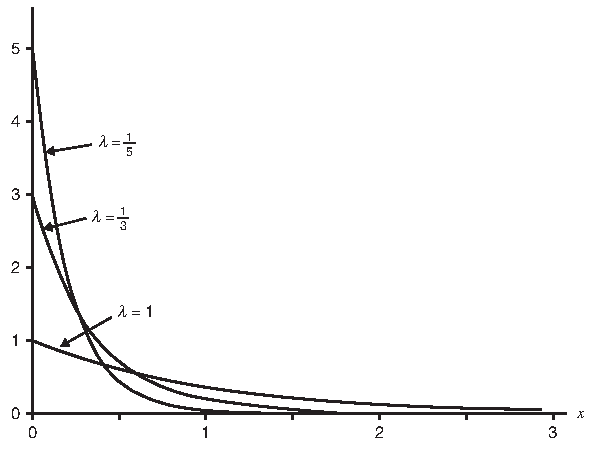
\includegraphics[width=.74\textwidth]{assets/chapter2/fig2-3-1.pdf}
\caption{$\lambda=1,\frac13,\frac15$ 时的指数密度.}\label{fig:2.3.1}
\end{figure}
\begin{example}[指数分布的方差]\label{ex:2.3.3}\index{SI0297@方差}
设 $X$ 具有\autoref{ex:2.2.2}中定义的 $\operatorname{exponential}(\lambda)$ 分布. 在那里我们算出了 $\mathrm EX=\lambda$，现在可以计算方差：
$$\begin{aligned}
\operatorname{Var}X&=\mathrm E(X-\lambda)^2=\int_0^\infty(x-\lambda)^2\frac1\lambda e^{-x/\lambda}\,dx\\
&=\int_0^\infty(x^2-2x\lambda+\lambda^2)\frac1\lambda e^{-x/\lambda}\,dx.
\end{aligned}$$
为了完成积分，可以对各项分别积分，对含有 $x$ 和 $x^2$ 的项使用分部积分. 这样就得到 $\operatorname{Var}X=\lambda^2$.
\end{example}
可见，指数分布的方差与参数 $\lambda$ 直接相关. \autoref{fig:2.3.1}给出了不同 $\lambda$ 值对应的几个指数分布. 注意，$\lambda$ 越小，分布就越集中在均值周围. 指数分布的方差作为 $\lambda$ 的函数所表现出的性质，是下列定理所概括的方差性质的一个特殊情形.
\begin{theorem}\label{thm:2.3.4}\index{SI1066@性质}
如果随机变量 $X$ 的方差有限，那么对任意常数 $a$ 和 $b$，
$$\operatorname{Var}(aX+b)=a^2\operatorname{Var}X.$$
\end{theorem}
\begin{proof}
由定义，
$$\begin{aligned}
\operatorname{Var}(aX+b)&=\mathrm E((aX+b)-\mathrm E(aX+b))^2\\
&=\mathrm E(aX-a\mathrm EX)^2&&\text{（$\mathrm E(aX+b)=a\mathrm EX+b$）}\\
&=a^2\mathrm E(X-\mathrm EX)^2\\
&=a^2\operatorname{Var}X.
\end{aligned}$$
\end{proof}

\sourcepageanchor{81}
有时使用方差的另一个公式更容易：
\begin{equation}\label{eq:2.3.1}
\operatorname{Var}X=\mathrm EX^2-(\mathrm EX)^2.
\end{equation}
只需注意下式便容易证明它：
$$\begin{aligned}
\operatorname{Var}X&=\mathrm E(X-\mathrm EX)^2=\mathrm E[X^2-2X\mathrm EX+(\mathrm EX)^2]\\
&=\mathrm EX^2-2(\mathrm EX)^2+(\mathrm EX)^2\\
&=\mathrm EX^2-(\mathrm EX)^2,
\end{aligned}$$
其中利用了 $\mathrm E(X\mathrm EX)=(\mathrm EX)(\mathrm EX)=(\mathrm EX)^2$，因为 $\mathrm EX$ 是常数. 现在用一个离散分布说明矩的计算.

\begin{example}[二项分布的方差]\label{ex:2.3.5}\index{SI0272@方差}
设 $X\sim\operatorname{binomial}(n,p)$，即
$$P(X=x)=\binom nx p^x(1-p)^{n-x},\qquad x=0,1,\ldots,n.$$
我们已经知道 $\mathrm EX=np$. 为计算 $\operatorname{Var}X$，先计算 $\mathrm EX^2$. 有
\begin{equation}\label{eq:2.3.2}
\mathrm EX^2=\sum_{x=0}^n x^2\binom nx p^x(1-p)^{n-x}.
\end{equation}
为求出这个级数之和，必须先对二项系数作变换，方法与求 $\mathrm EX$ 时类似（\autoref{ex:2.2.3}）. 写成
\begin{equation}\label{eq:2.3.3}
x^2\binom nx=x\frac{n!}{(x-1)!(n-x)!}=xn\binom{n-1}{x-1}.
\end{equation}
\eqref{eq:2.3.2}中 $x=0$ 对应的项为零，利用\eqref{eq:2.3.3}，得到
$$\begin{aligned}
\mathrm EX^2&=n\sum_{x=1}^n x\binom{n-1}{x-1}p^x(1-p)^{n-x}\\
&=n\sum_{y=0}^{n-1}(y+1)\binom{n-1}y p^{y+1}(1-p)^{n-1-y}&&\text{（令 $y=x-1$）}\\
&=np\sum_{y=0}^{n-1}y\binom{n-1}y p^y(1-p)^{n-1-y}\\
&\qquad+np\sum_{y=0}^{n-1}\binom{n-1}y p^y(1-p)^{n-1-y}.
\end{aligned}$$
现在容易看出，第一个和等于 $(n-1)p$，因为它是 $\operatorname{binomial}(n-1,p)$ 分布的均值；第二个和等于 $1$. 因此，
\begin{equation}\label{eq:2.3.4}
\mathrm EX^2=n(n-1)p^2+np.
\end{equation}
由\eqref{eq:2.3.1}，得到
$$\operatorname{Var}X=n(n-1)p^2+np-(np)^2=-np^2+np=np(1-p).$$
\end{example}

高阶矩的计算方式类似，但数学运算通常会变得相当复杂. 在应用中，有时会关心三阶或四阶矩；但从统计学角度看，通常没有多少理由考察更高阶的矩.

现在介绍与概率分布相关的一个新函数——矩母函数（moment generating function，mgf）. 顾名思义，矩母函数可以用来生成矩. 实际上，很多时候直接计算矩比使用矩母函数更容易. 然而，矩母函数的主要用途并不是生成矩，而是帮助刻画分布. 恰当地使用这一性质，可以得到极为有力的结果.

\sourcepageanchor{82}
\begin{definition}\label{def:2.3.6}\index{SI0689@矩母函数}\index{SI0720@邻域}
设 $X$ 是具有累积分布函数 $F_X$ 的随机变量. $X$（或 $F_X$）的矩母函数，记为 $M_X(t)$，定义为
$$M_X(t)=\mathrm Ee^{tX},$$
前提是这个期望对 $0$ 的某个邻域内的 $t$ 存在. 也就是说，存在 $h>0$，使得对所有 $-h<t<h$，$\mathrm Ee^{tX}$ 都存在. 如果这个期望在 $0$ 的任何邻域内都不是处处存在的，就说矩母函数不存在.
\end{definition}
更明确地说，$X$ 的矩母函数可写为
$$M_X(t)=\int_{-\infty}^\infty e^{tx}f_X(x)\,dx,\qquad X\text{ 连续},$$
或者
$$M_X(t)=\sum_x e^{tx}P(X=x),\qquad X\text{ 离散}.$$
很容易看出矩母函数如何生成矩. 我们将这一结果概括为下列定理.
\begin{theorem}\label{thm:2.3.7}
如果 $X$ 的矩母函数为 $M_X(t)$，那么
$$\mathrm EX^n=M_X^{(n)}(0),$$
其中定义
$$M_X^{(n)}(0)=\left.\frac{d^n}{dt^n}M_X(t)\right|_{t=0}.$$
也就是说，$n$ 阶矩等于 $M_X(t)$ 的 $n$ 阶导数在 $t=0$ 处的值.
\end{theorem}
\begin{proof}
假定可以在积分号下求导（见\autoref{sec:2.4}），则
$$\begin{aligned}
\frac d{dt}M_X(t)&=\frac d{dt}\int_{-\infty}^\infty e^{tx}f_X(x)\,dx\\
&=\int_{-\infty}^\infty\left(\frac d{dt}e^{tx}\right)f_X(x)\,dx\\
&=\int_{-\infty}^\infty(xe^{tx})f_X(x)\,dx\\
&=\mathrm EXe^{tX}.
\end{aligned}$$
于是，
$$\left.\frac d{dt}M_X(t)\right|_{t=0}=\left.\mathrm EXe^{tX}\right|_{t=0}=\mathrm EX.$$
用类似方式可得
$$\left.\frac{d^n}{dt^n}M_X(t)\right|_{t=0}=\left.\mathrm EX^ne^{tX}\right|_{t=0}=\mathrm EX^n.$$
\end{proof}

\begin{example}[伽马分布的矩母函数]\label{ex:2.3.8}\index{SI0308@矩母函数}
在\autoref{ex:2.1.6}中，我们遇到了伽马密度的一种特殊情形；一般的伽马密度为
$$f(x)=\frac1{\Gamma(\alpha)\beta^\alpha}x^{\alpha-1}e^{-x/\beta},\qquad0<x<\infty,\quad\alpha>0,\quad\beta>0,$$
\sourcepageanchor{83}
其中 $\Gamma(\alpha)$ 表示伽马函数（gamma function），它的一些性质将在\autoref{sec:3.3}中给出. 矩母函数为
\begin{equation}\label{eq:2.3.5}
\begin{aligned}
M_X(t)&=\frac1{\Gamma(\alpha)\beta^\alpha}\int_0^\infty e^{tx}x^{\alpha-1}e^{-x/\beta}\,dx\\
&=\frac1{\Gamma(\alpha)\beta^\alpha}\int_0^\infty x^{\alpha-1}e^{-(\frac1\beta-t)x}\,dx\\
&=\frac1{\Gamma(\alpha)\beta^\alpha}\int_0^\infty x^{\alpha-1}e^{-x/(\frac\beta{1-\beta t})}\,dx.
\end{aligned}
\end{equation}
现在可以认出，\eqref{eq:2.3.5}中的被积函数是另一个伽马密度的核（kernel）\index{SI0595@核}\semanticindexanchor{595:83}. （函数的核是函数的主要部分，即忽略常数后余下的部分.）利用对任意正常数 $a,b$，
$$f(x)=\frac1{\Gamma(a)b^a}x^{a-1}e^{-x/b}$$
是概率密度函数这一事实，有
$$\int_0^\infty\frac1{\Gamma(a)b^a}x^{a-1}e^{-x/b}\,dx=1,$$
从而
\begin{equation}\label{eq:2.3.6}
\int_0^\infty x^{a-1}e^{-x/b}\,dx=\Gamma(a)b^a.
\end{equation}
将\eqref{eq:2.3.6}应用于\eqref{eq:2.3.5}，得到
$$M_X(t)=\frac1{\Gamma(\alpha)\beta^\alpha}\Gamma(\alpha)
\left(\frac\beta{1-\beta t}\right)^\alpha
=\left(\frac1{1-\beta t}\right)^\alpha,\qquad t<\frac1\beta.$$
如果 $t\ge1/\beta$，\eqref{eq:2.3.5}被积函数中的 $(1/\beta)-t$ 非正，而\eqref{eq:2.3.6}中的积分为无穷大. 因此，伽马分布的矩母函数只在 $t<1/\beta$ 时存在. （我们将在\autoref{sec:3.3}中更详细地讨论伽马函数.）

伽马分布的均值为
$$\mathrm EX=\left.\frac d{dt}M_X(t)\right|_{t=0}
=\left.\frac{\alpha\beta}{(1-\beta t)^{\alpha+1}}\right|_{t=0}=\alpha\beta.$$
其他矩可用类似方式计算.
\end{example}

\begin{example}[二项分布的矩母函数]\label{ex:2.3.9}\index{SI0265@矩母函数}
作为计算矩母函数的第二个例子，我们考虑一个离散分布——二项分布. $\operatorname{binomial}(n,p)$ 的概率质量函数由\eqref{eq:2.1.3}给出，因此
$$M_X(t)=\sum_{x=0}^n e^{tx}\binom nx p^x(1-p)^{n-x}
=\sum_{x=0}^n\binom nx(pe^t)^x(1-p)^{n-x}.$$
二项式公式（见\autoref{thm:3.2.2}）给出
\begin{equation}\label{eq:2.3.7}
\sum_{x=0}^n\binom nx u^xv^{n-x}=(u+v)^n.
\end{equation}
因此，令 $u=pe^t$、$v=1-p$，得到
$$M_X(t)=[pe^t+(1-p)]^n.$$
\end{example}

\sourcepageanchor{84}
\begin{figure}[htbp]\centering
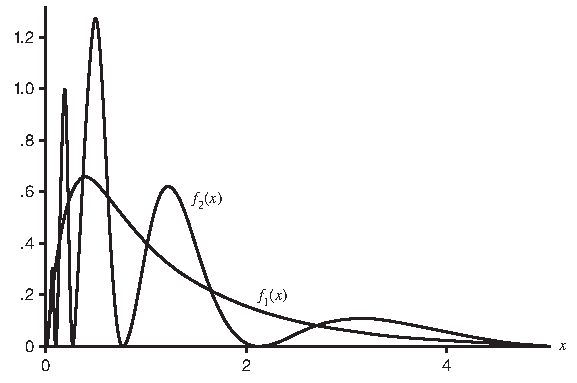
\includegraphics[width=.76\textwidth]{assets/chapter2/fig2-3-2.pdf}
\caption{具有相同各阶矩的两个概率密度函数：$f_1(x)=\frac1{\sqrt{2\pi}x}e^{-(\log x)^2/2}$，$f_2(x)=f_1(x)[1+\sin(2\pi\log x)]$.}\label{fig:2.3.2}
\end{figure}
如前所述，矩母函数的主要用途并不是生成矩，而在于它在许多情况下能够刻画分布. 不过，用矩来刻画分布会遇到一些技术困难，现在就来研究这些困难.

如果矩母函数存在，它就刻画了无穷多个矩. 一个自然的问题是：刻画这无穷多个矩，是否就唯一确定了分布函数？遗憾的是，答案是否定的. 仅仅刻画所有矩，不足以唯一确定分布，因为两个不同的随机变量可能具有相同的各阶矩.

\begin{example}[矩的不唯一性]\label{ex:2.3.10}\index{SI0334@矩}\index{SI0698@非唯一性}
考虑两个概率密度函数
$$\begin{aligned}
f_1(x)&=\frac1{\sqrt{2\pi}x}e^{-(\log x)^2/2},&0\le x<\infty,\\
f_2(x)&=f_1(x)[1+\sin(2\pi\log x)],&0\le x<\infty.
\end{aligned}$$
（密度 $f_1$ 是对数正态密度（lognormal pdf）的一种特殊情形.）
可以证明，若 $X_1\sim f_1(x)$，则
$$\mathrm EX_1^r=e^{r^2/2},\qquad r=0,1,\ldots,$$
所以 $X_1$ 的所有阶矩都存在. 现设 $X_2\sim f_2(x)$，有
$$\begin{aligned}
\mathrm EX_2^r&=\int_0^\infty x^rf_1(x)[1+\sin(2\pi\log x)]\,dx\\
&=\mathrm EX_1^r+\int_0^\infty x^rf_1(x)\sin(2\pi\log x)\,dx.
\end{aligned}$$
但是，变换 $y=\log x-r$ 表明，最后的积分是一个奇函数在 $(-\infty,\infty)$ 上的积分，因而对 $r=0,1,\ldots$ 都等于 $0$. 所以，尽管 $X_1$ 与 $X_2$ 的密度不同，它们的所有阶矩却都相同. 两个密度画在\autoref{fig:2.3.2}中.

细节见\autoref{exercise:2.35}；有关矩母函数和分布的更多内容，另见\autoref{exercise:2.34}、\autoref{exercise:2.36}及\autoref{exercise:2.37}.
\end{example}

\sourcepageanchor{85}
如果随机变量具有有界支撑，就不会出现矩的唯一性问题. 此时，无穷矩序列确实唯一确定分布（例如，见 \hyperref[bib:source33]{Billingsley 1995}，第~30~节）. 而且，如果矩母函数在零的某个邻域内存在，无论支撑集怎样，分布都被唯一确定. 因而，所有阶矩都存在与矩母函数存在并不等价. 下列定理说明如何刻画分布.
\needspace{6\baselineskip}
\begin{theorem}\label{thm:2.3.11}\index{SI0691@同分布}\index{SI0870@矩}
设 $F_X(x)$ 和 $F_Y(y)$ 是两个各阶矩都存在的累积分布函数.
\begin{enumerate}
\item[(a)] 若 $X$ 和 $Y$ 具有有界支撑，则对所有 $u$ 有 $F_X(u)=F_Y(u)$，当且仅当对所有整数 $r=0,1,2,\ldots$ 有 $\mathrm EX^r=\mathrm EY^r$.
\item[(b)] 若矩母函数存在，并且对 $0$ 的某个邻域内的所有 $t$ 有 $M_X(t)=M_Y(t)$，则对所有 $u$ 有 $F_X(u)=F_Y(u)$.
\end{enumerate}
\end{theorem}
下一个定理讨论一个收敛的矩母函数序列，我们不再单独处理有界支撑的情形. 注意，如果极限矩母函数在 $0$ 的某个邻域内存在，则唯一性假设自动满足（\hyperref[sec:2.6.1]{杂录~2.6.1}）.
\begin{theorem}[矩母函数的收敛]\label{thm:2.3.12}\index{SI0690@收敛}
设 $\{X_i,\ i=1,2,\ldots\}$ 是随机变量序列，每个随机变量的矩母函数为 $M_{X_i}(t)$. 再设
$$\lim_{i\to\infty}M_{X_i}(t)=M_X(t),\qquad\text{对 $0$ 的某个邻域内的所有 $t$},$$
而 $M_X(t)$ 是一个矩母函数. 则存在唯一的累积分布函数 $F_X$，其矩由 $M_X(t)$ 确定；并且对 $F_X(x)$ 连续的所有 $x$，有
$$\lim_{i\to\infty}F_{X_i}(x)=F_X(x).$$
也就是说，矩母函数在 $|t|<h$ 时收敛到一个矩母函数，蕴含累积分布函数的收敛.
\end{theorem}
\autoref{thm:2.3.11}和\autoref{thm:2.3.12}的证明依赖于拉普拉斯变换（Laplace transform）理论. （经典参考文献是 \hyperref[bib:source329]{Widder (1946)}，\hyperref[bib:source119]{Feller (1971)} 也对拉普拉斯变换作了全面介绍.）$M_X(t)$ 的定义式，即
\begin{equation}\label{eq:2.3.8}\index{SI0601@拉普拉斯变换}
M_X(t)=\int_{-\infty}^\infty e^{tx}f_X(x)\,dx,
\end{equation}
定义了一个拉普拉斯变换（$M_X(t)$ 是 $f_X(x)$ 的拉普拉斯变换）. 拉普拉斯变换的一个关键性质是唯一性. 若对满足 $|t|<h$ 的所有 $t$，\eqref{eq:2.3.8}都成立，其中 $h$ 为某个正数，那么给定 $M_X(t)$ 后，只有一个函数 $f_X(x)$ 满足\eqref{eq:2.3.8}. 有了这个事实，前面两个定理就相当合理了. 尽管它们的严格证明没有超出本书的范围，但证明较为技术化，并不能带来真正的理解，因此这里略去.

矩序列可能不具有唯一性，是件麻烦事. 如果证明某个矩序列收敛，我们还不能正式断言随机变量收敛. 为了得出这一结论，还必须核实矩序列的唯一性，而这通常是一项可怕的工作（\hyperref[sec:2.6.1]{杂录~2.6.1}）. 但是，如果矩母函数序列在 $0$ 的某个邻域内收敛，那么随机变量就收敛. 因此，矩母函数的收敛可以视为随机变量序列收敛的一个充分但非必要条件.

\begin{example}[泊松近似]\label{ex:2.3.13}\index{SI0060@以泊松近似二项}
初等统计课程通常介绍的一种近似是：二项概率（见\autoref{ex:2.3.5}）可以用通常更容易计算的泊松概率（Poisson probabilities）来近似. 二项分布由两个量 $n$ 和 $p$ 刻画. 通常的说法是，当“$n$ 大而 $np$ 小”时，泊松近似有效，有时还会给出经验规则.
\sourcepageanchor{86}
$\operatorname{Poisson}(\lambda)$ 的概率质量函数为
$$P(X=x)=\frac{e^{-\lambda}\lambda^x}{x!},\qquad x=0,1,2,\ldots,$$
其中 $\lambda$ 为正常数. 这个近似是说，如果 $X\sim\operatorname{binomial}(n,p)$，$Y\sim\operatorname{Poisson}(\lambda)$，且 $\lambda=np$，则对大的 $n$ 和小的 $np$，
\begin{equation}\label{eq:2.3.9}
P(X=x)\approx P(Y=x).
\end{equation}
现在证明矩母函数收敛，从而为这一近似提供依据. 回顾
\begin{equation}\label{eq:2.3.10}
M_X(t)=[pe^t+(1-p)]^n.
\end{equation}
对于 $\operatorname{Poisson}(\lambda)$ 分布，可以算出（见\autoref{exercise:2.33}）
$$M_Y(t)=e^{\lambda(e^t-1)},$$
而如果定义 $p=\lambda/n$，当 $n\to\infty$ 时就有 $M_X(t)\to M_Y(t)$. \eqref{eq:2.3.9}中近似的有效性于是由\autoref{thm:2.3.12}得到.

我们先稍作离题，介绍一个在统计学中有广泛应用的重要极限结果. 这个引理的证明可在许多标准微积分教材中找到.
\begin{lemma}\label{lem:2.3.14}\index{SI0372@矩母函数}
设数列 $a_1,a_2,\ldots$ 收敛到 $a$，即 $\lim_{n\to\infty}a_n=a$. 则
$$\lim_{n\to\infty}\left(1+\frac{a_n}n\right)^n=e^a.$$
\end{lemma}
回到例子，有
$$\begin{aligned}
M_X(t)&=[pe^t+(1-p)]^n\\
&=\left[1+\frac1n(e^t-1)(np)\right]^n
=\left[1+\frac1n(e^t-1)\lambda\right]^n,
\end{aligned}$$
因为 $\lambda=np$. 现在令 $a_n=a=(e^t-1)\lambda$，应用\autoref{lem:2.3.14}，得到
$$\lim_{n\to\infty}M_X(t)=e^{\lambda(e^t-1)}=M_Y(t),$$
即泊松分布的矩母函数.

即使 $p$ 和 $n$ 的大小适中，泊松近似也可能相当好. \autoref{fig:2.3.3}给出了一个二项质量函数及其 $\lambda=np$ 的泊松近似. 这个近似看起来令人满意.
\end{example}

本节最后给出关于矩母函数的一个有用结果.
\begin{theorem}\label{thm:2.3.15}\index{SI0693@性质}
对任意常数 $a,b$，随机变量 $aX+b$ 的矩母函数为
$$M_{aX+b}(t)=e^{bt}M_X(at).$$
\end{theorem}
\begin{proof}
由定义，
$$\begin{aligned}
M_{aX+b}(t)&=\mathrm E\bigl(e^{(aX+b)t}\bigr)\\
&=\mathrm E\bigl(e^{(aX)t}e^{bt}\bigr)&&\text{（指数函数的性质）}\\
&=e^{bt}\mathrm E\bigl(e^{(at)X}\bigr)&&\text{（$e^{bt}$ 是常数）}\\
&=e^{bt}M_X(at),&&\text{（矩母函数的定义）}
\end{aligned}$$
定理得证.
\end{proof}
\sourcepageanchor{87}
\begin{figure}[htbp]\centering
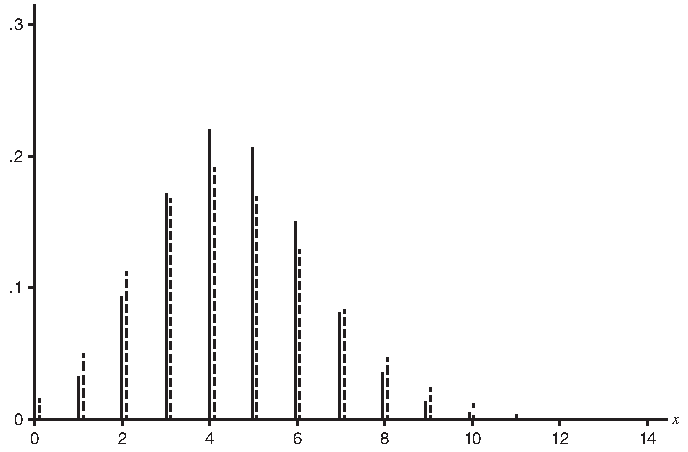
\includegraphics[width=.85\textwidth]{assets/chapter2/fig2-3-3.pdf}
\caption{二项分布（实线）的泊松近似（虚线），$n=15$，$p=.3$.}\label{fig:2.3.3}
\end{figure}
